\subsection{Example}\label{sec:example}

In this section, we present an illustrative pipeline template, concentrating on the policy annotations.
The pipeline template consists of six stages, and each stage is noted with a policy.
All these policies are outlined in \cref{tab:anonymization}.
Additionally, \cref{tab:dataset} shows a sample of the dataset.
It is assumed that the Connecticut Prison (CTP) is the data owner, with partnerships with two other facilities, namely New York Prison and
New Hampshire Prison.

In the following we will make reference to three different type of anonymization:
\begin{enumerate*}[label=\roman*)]
  \item \emph{none} (\tf{1}): no anonymization is performed;
  \item \emph{light} (\tf{2}): the data is partially anonymized, only the first name and last name are anonymized;
  \item \emph{full} (\tf{3}): the data is fully anonymized: first name, last name, identifier and age are anonymized.
\end{enumerate*}
Let us consider the pipeline template \tChartFunction in \cref{sec:example},
% 1° NODO %
The first vertex is responsible for data anonymization and is associated with three policies (\p{1},\p{2},\p{3}).
During the node execution, the policies are assessed:
if the service profile matches with the data owner ($owner = ``CTP"$), \p{1} is satisfied and the data is not anonymized (\tf{1});
if the service profile matches with a partner of the owner ($owner = ``CTP"$), \p{2} is satisfied and the data is partially anonymized (\tf{2});
if the service profile doesn't match with a partner nor with the owner ($owner = ``CTP"$), \p{3} is satisfied and the data is fully anonymized (\tf{3}).
% 2° NODO %
The second vertex is responsible for enriching the data.
The service downloads the dataset from partner facilities and enhances the dataset of the Connecticut facility.
The policies are consistent with those of the first stage (\p{1},\p{2},p{3}).
if the service is \hl{made} by the data owner ($\langle owner = ``CTP" \rangle$), the owner dataset remains unaltered (\tf{0}), whereas the partner dataset is partially anonymized .
if the service is \hl{made} by their partners ($\langle owner = ``CTP" \rangle$), the owner dataset is partially anonymized as well as the partner dataset.
if the service is \hl{made} by a third party ($\langle owner = ``CTP" \rangle$), the owner dataset is fully anonymized as well as the partner dataset.
% 3° NODO %
The third vertex, is responsible for data analysis and statistics,
it adopts policies analogous to the first stage. The logic remains consistent:
if the service profile matches with the data owner ($\langle owner = ``CTP" \rangle$), \p{1} is satisfied and the data computation is made on non anonymized data (\tf{1});
if the service profile matches with a partner of the owner ($\langle owner = partner(``CTP") \rangle$), \p{2} is satisfied and the data computation is made on partially anonymized data (\tf{2});
if the service profile doesn't match with a partner nor with the owner ($\langle owner = ``any" \rangle$), \p{3} is satisfied and the data computation is made on fully anonymized data (\tf{3}).
% 4° NODO %
The fourth vertex is responsible for machine learning tasks:
The policy guidelines recommend anonymizing all datasets to prevent personal identifiers from entering into the machine learning algorithm/model (\tf{3}).
% 5° NODO %
The fifth vertex manages data storage.
If the service is within the facility itself ($\langle service,region=FACILITY"\rangle$), \p{5} is satisfied, resulting in data anonymization (\tf{1}).
Otherwise, if the service is in a partner region ($\langle service,region={CT,NY,NH}"\rangle$), the data undergo partial anonymization (\tf{2}).
% 6° NODO %
The sixth vertex is responsible for data visualization.
As stated in policy annotation \p{6}, if the user is member of the facility itself, the data are not anonymized (\tf{1}).
If the user is member of a partner facility, the data are  partially anonymized (\tf{2}).
If the user is not member of the facility nor a partner, the data are fully anonymized (\tf{3}).


In summary, this section has delineated a comprehensive pipeline template.
This illustrative pipeline serves as a blueprint, highlighting the role of policy implementation in safeguarding data protection across diverse operational stages.
\begin{table*}[ht!]
  \centering
  \caption{Anonymization policies}
  \label{tab:anonymization}
  \bgroup
  \def\arraystretch{1.5}

  \begin{tabular}[t]{c|c|l}
    \textbf{Vertex}      & \textbf{Policy} & \policy{subject}{object}{action}{environment}{transformation}                                   \\ \hline

    \vi{1},\vi{2},\vi{3} & $\p{1}$         & \policy{$\langle service,owner=``CTP"\rangle$}{dataset}{READ}{ANY}{ \tf{1}    }                 \\
    \vi{1},\vi{2},\vi{3} & $\p{2}$         & \policy{$\langle service,owner=partner(``CTP") \rangle$}{dataset}{READ}{ANY}{   \tf{2} }        \\
    \vi{1},\vi{2},\vi{3} & $\p{3}$         & \policy{$\langle service,owner=``Any"$}{dataset}{READ}{ANY}{    \tf{3}  }                       \\
    \vi{4}               & $\p{4}$         & \policy{ANY}{dataset}{READ}{ANY}{    \tf{3}  }                                                  \\
    \vi{5}               & $\p{5}$         & \policy{$\langle service,region=``FACILITY"\rangle$}{dataset}{WRITE}{ANY}{ \tf{1}    }          \\
    \vi{5}               & $\p{6}$         & \policy{$\langle service,region=``\{CT,NY,NH\}"\rangle$}{dataset}{WRITE}{ANY}{   \tf{2} }       \\
    \vi{6}               & $\p{7}$         & \policy{$\langle user,role=   ``Connecticut Prison Officer"$}{dataset} {READ}{ANY}{ \tf{1}    } \\
    \vi{6}               & $\p{7}$         & \policy{$\langle user,role=   ``Partener Prison Officer"$}{dataset} {READ}{ANY}{   \tf{2} }     \\
    \vi{6}               & $\p{8}$         & \policy{$\langle user,role=   ``Any"$}{dataset} {READ}{ANY}{    \tf{3}  }                       \\
  \end{tabular}
  \begin{tabular}[t]{c|c|c}
    \textbf{\tf{i}} & \textbf{Anonymization} & \textbf{Columns Anonymized}                 \\\hline
    \tf{1}          & none                   & $\varnothing$                               \\
    \tf{2}          & light                  & \{ FIRST NAME, LAST NAME \}                 \\
    \tf{3}          & full                   & \{ FIRST NAME, LAST NAME, IDENTIFIER,AGE \} \\
  \end{tabular}

  \egroup
\end{table*}
\vspace{2em}
\begin{table*}[!ht]
  \caption{Dataset sample}
  \label{tab:dataset}
  \centering
  \begin{adjustbox}{max totalsize={.99\linewidth}{\textheight},center}
    \bgroup
    \def\arraystretch{1.5}
    \begin{tabular}{|l|l|l|l|l|l|l|l|l|l|l|l|}
      \hline
      \textbf{DOWNLOAD DATE} & \textbf{IDENTIFIER} & \textbf{FIRST NAME} & \textbf{LAST NAME} & \textbf{LAD} & \textbf{RACE} & \textbf{GENDER} & \textbf{AGE} & \textbf{BOND} & \textbf{OFFENSE}     & \textbf{\dots} \\ \hline
      05/15/2020             & ZZHCZBZZ            & ROBERT              & PIERCE             & 08/16/2018   & BLACK         & M               & 27           & 150000        & CRIMINAL POSS \dots  & \dots          \\ \hline
      05/15/2020             & ZZHZZRLR            & KYLE                & LESTER             & 03/28/2019   & HISPANIC      & M               & 41           & 30100         & VIOLATION OF P\dots  & \dots          \\ \hline
      05/15/2020             & ZZSRJBEE            & JASON               & HAMMOND            & 04/03/2020   & HISPANIC      & M               & 21           & 150000        & CRIMINAL ATTEM\dots  & \dots          \\ \hline
      05/15/2020             & ZZHBJLRZ            & ERIC                & TOWNSEND           & 01/15/2020   & WHITE         & M               & 36           & 50500         & CRIM VIOL OF P\dots  & \dots          \\ \hline
      05/15/2020             & ZZSRRCHH            & MICHAEL             & WHITE              & 12/26/2018   & HISPANIC      & M               & 29           & 100000        & CRIMINAL ATTEM\dots  & \dots          \\ \hline
      05/15/2020             & ZZEJCZWW            & JOHN                & HARPER             & 01/03/2020   & WHITE         & M               & 54           & 100000        & CRIM VIOL OF P\dots  & \dots          \\ \hline
      05/15/2020             & ZZHJBJBR            & KENNETH             & JUAREZ             & 03/19/2020   & HISPANIC      & M               & 35           & 100000        & CRIM VIOL ST C\dots  & \dots          \\ \hline
      05/15/2020             & ZZESESZW            & MICHAEL             & SANTOS             & 12/03/2018   & WHITE         & M               & 55           & 50000         & ASSAULT 2ND, V\dots  & \dots          \\ \hline
      05/15/2020             & ZZRCSHCZ            & CHRISTOPHER         & JONES              & 05/13/2020   & BLACK         & M               & 43           & 10000         & INTERFERING WIT\dots & \dots          \\ \hline
    \end{tabular}
    \egroup
  \end{adjustbox}

\end{table*}
\begin{figure}[ht!]
  \centering
  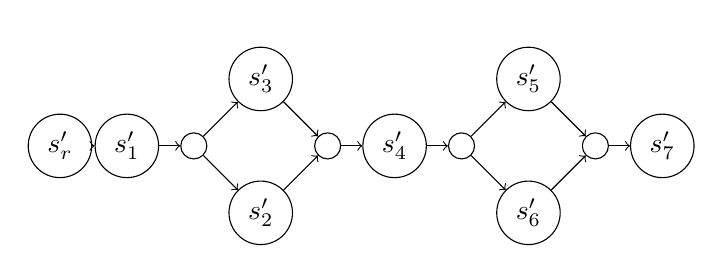
\begin{tikzpicture}[scale=0.85]
    \node[draw, circle] (node1) at (0,0) {$s^\prime_r$};
    \node[draw, circle] (node2) at (1,0) {$s^\prime_1$};
    \node[draw, circle] (node3) at (2,0) {$\timesOperator$};
    \node[draw, circle] (node4) at (3,-1) {$s^\prime_2$};
    \node[draw, circle] (node5) at (3,1) {$s^\prime_3$};
    \node[draw, circle] (node6) at (4,0) {$\timesOperator$};
    \node[draw, circle] (node65) at (5,0) {$s^\prime_4$};
    \node[draw, circle] (node7) at (6,0) {$\plusOperator$};
    \node[draw, circle] (node8) at (7,1) {$s^\prime_5$};
    \node[draw, circle] (node9) at (7,-1) {$s^\prime_6$};
    \node[draw, circle] (node10) at (8,0) {$\plusOperator$};
    \node[draw, circle] (node11) at (9,0) {$s^\prime_7$};
    % Text on top
    \node[above] at (node1.north) { \footnotesize$\instanceChartAnnotation$};
    \node[above] at (node2.north) { \footnotesize$\instanceChartAnnotation$};
    \node[above] at (node3.north) {};
    \node[above] at (node4.north) { \footnotesize$\instanceChartAnnotation$};
    \node[above] at (node5.north) { \footnotesize$\instanceChartAnnotation$};
    \node[above] at (node65.north) { \footnotesize$\instanceChartAnnotation$};
    \node[above] at (node8.north) { \footnotesize$\instanceChartAnnotation$};
    \node[above] at (node9.north) { \footnotesize$\instanceChartAnnotation$};
    \node[above] at (node11.north) { \footnotesize$\instanceChartAnnotation$};
    % Connection
    \draw[->] (node1) -- (node2);
    \draw[->] (node2) -- (node3);
    \draw[->] (node3) -- (node4);
    \draw[->] (node3) -- (node5);
    \draw[->] (node5) -- (node6);
    \draw[->] (node4) -- (node6);
    \draw[->] (node6) -- (node65);
    \draw[->] (node65) -- (node7);
    \draw[->] (node7) -- (node8);
    \draw[->] (node7) -- (node9);
    \draw[->] (node8) -- (node10);
    \draw[->] (node9) -- (node10);
    \draw[->] (node10) -- (node11);
  \end{tikzpicture}
  \caption{Service composition instance}
  \label{fig:service_composition_instance}
\end{figure}
